\documentclass[11pt]{article}

\usepackage[margin=1in]{geometry}
\usepackage{amsmath, amssymb}
\usepackage{graphicx}
\usepackage{listings}
\usepackage{xcolor}
\usepackage{hyperref}
\usepackage{booktabs}

\usepackage{minted}
\usepackage[capitalise,noabbrev]{cleveref}

\lstset{
    basicstyle=\ttfamily\small,
    breaklines=true,
    frame=single,
    numbers=left,
    numberstyle=\tiny,
    keywordstyle=\color{blue},
    commentstyle=\color{gray},
    tabsize=4
}

\title{High Performance Parallel Computing \\ Homework 1}
\author{Liam Pohlmann, Alex Shaffer}
\date{\today}

\begin{document}

\maketitle

\section{Problem 1}

Using the provided MatLab code, MatLab version R2025b was run on the \texttt{eng-partition} on a single node with a single single task and a single CPU per task.

\inputminted{batch}{../q1_results/matlab_results/batch_matlab.sh}

This produced the results seen in \cref{fig:matlab_gflops}.

\begin{figure}
    \centering
    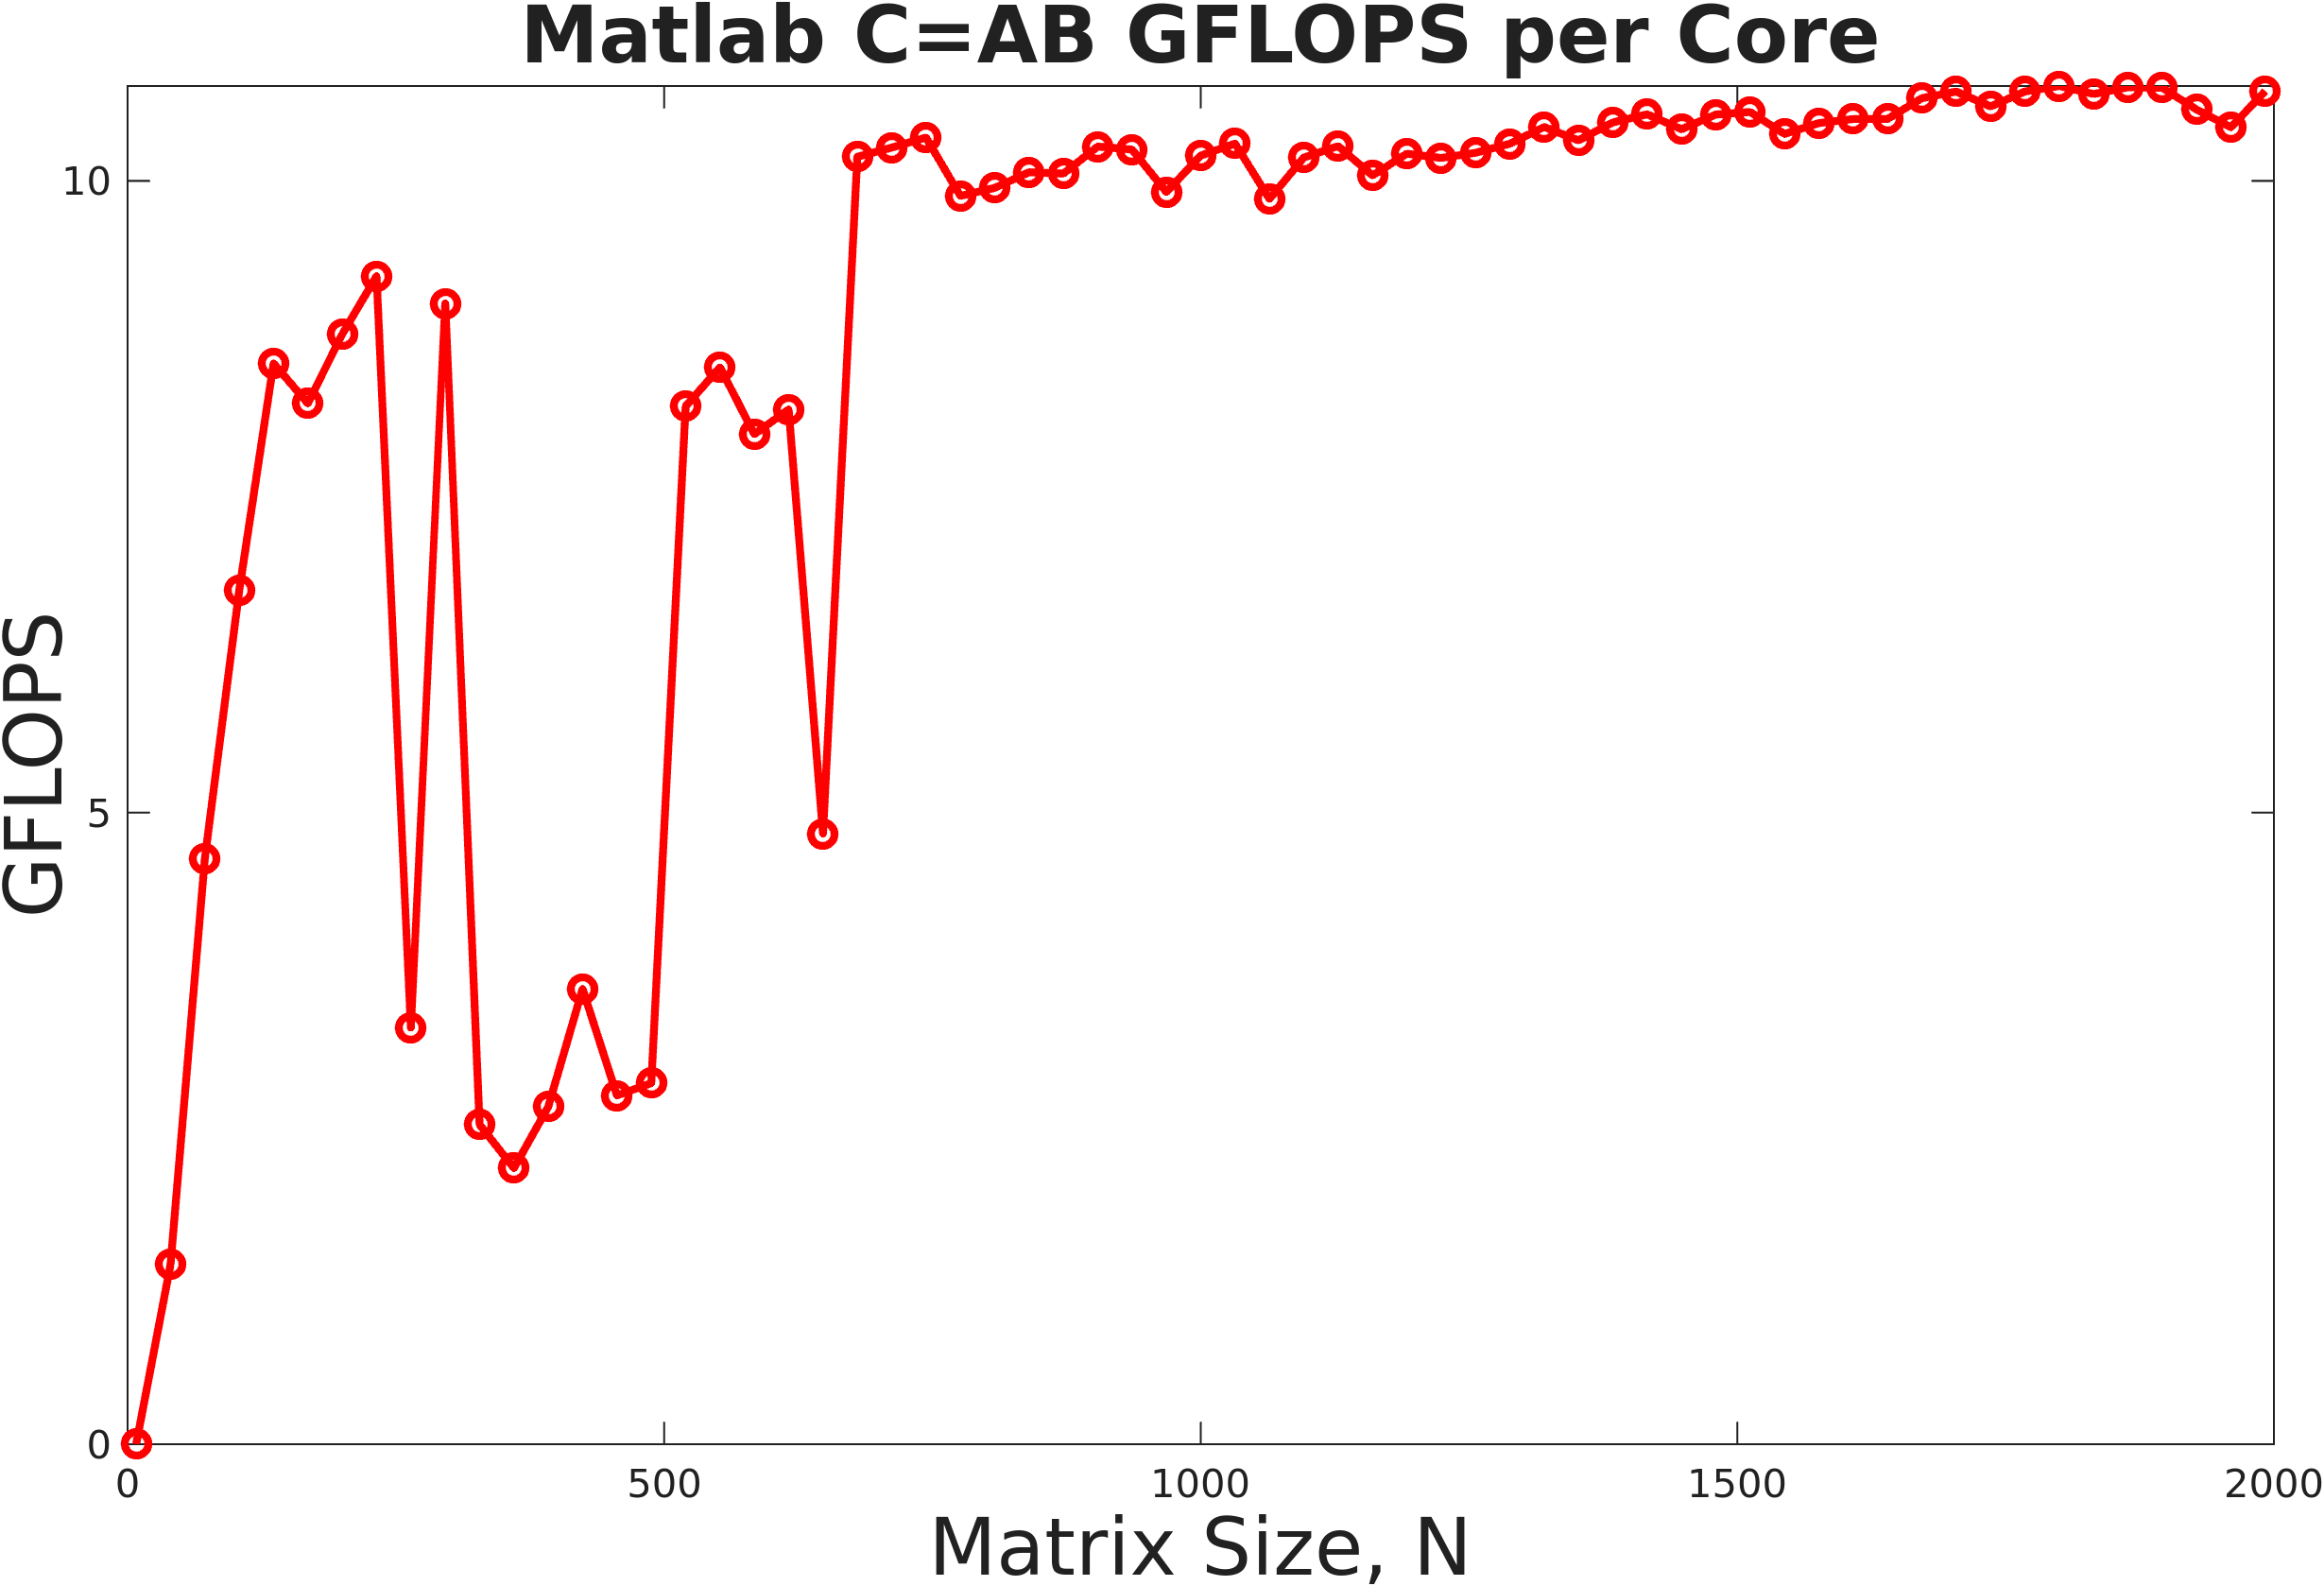
\includegraphics[width=0.8\textwidth]{../q1_results/matlab_results/octave_gflops.png}
    \label{fig:matlab_gflops}
    \caption{}
\end{figure}


\section{Problem 2}

\end{document}
